\subsubsection{Leistungsfähigkeit bei unterschiedlichen Geschwindigkeiten}
%In diesem Abschnitt soll untersucht werden, ob eine Reduzierung der Geschwindigkeit positive Auswirkungen auf die Zuverlässigkeit von Bildverarbeitung und Regelung besitzt.

Nachdem eine passende Einstellung der Regel-und Bildverarbeitungsfrequenz gefunden wurde, soll nun das Fahren mit höheren Geschwindigkeiten betrachtet werden. Neben der normalen Sichtprüfung der Funktionalität der Fahrspurverfolgung wurden die Anzahl der zur Zielpunktbestimmung genutzten Weltkartenpunkte pro Regelung und der prozentuale Anteil an nicht bestimmten Zielpunkten zur Untersuchung herangezogen. 

Zur besseren Vergleichbarkeit der Messergebnisse wurden die Daten für je eine entgegen des Uhrzeigersinnes gefahrene Runde mit \SI{3}{\hertz} Bildverarbeitungsfrequenz aufgenommen.

\begin{figure}[h] % [htb]
	\centering
	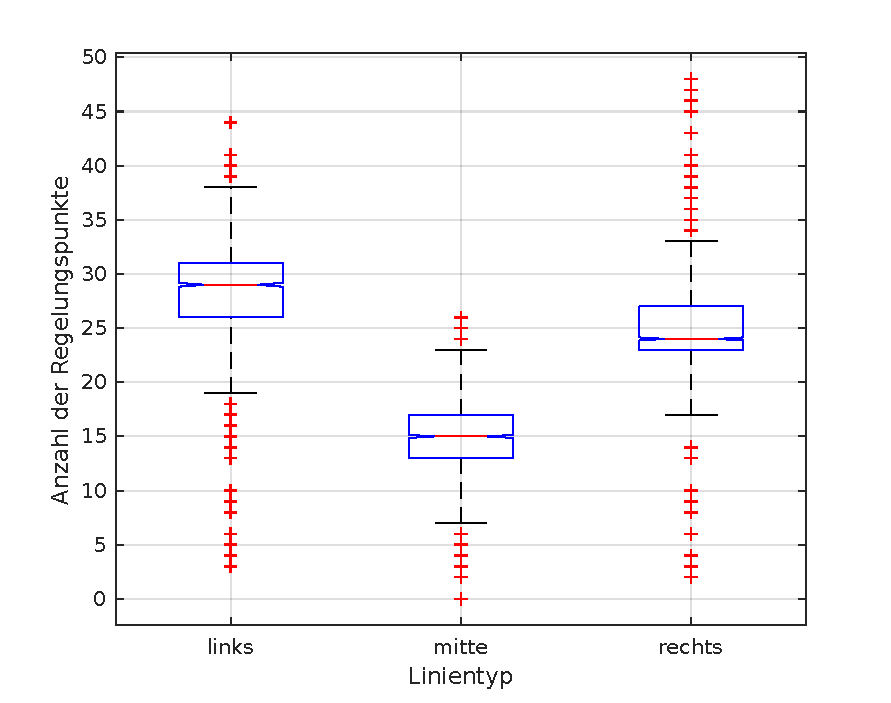
\includegraphics[width=0.9\textwidth]{evaluation_riverflow_regelungspunkte_je_linie_0.2m_s_3Hz.pdf}
	\caption{Anzahl der jeweiligen zur Regelung genutzten Punkte aus der Weltkarte bei \( \gls{lat:velocity} = \SI{0,2}{\metre\per\second} \)}
	\label{fig:evaluation:riverflow:regelungspunkte_je_linie}
\end{figure}

Abbildung~\ref{fig:evaluation:riverflow:regelungspunkte_je_linie} zeigt exemplarisch für die Geschwindigkeit \( \gls{lat:velocity} = \SI{0,2}{\metre\per\second} \) den  Anteil jeweiliger Linienpunkttypen zur Zielpunktberechnung. Es fällt sogleich auf, dass die Mittellinie einen weniger starken Einfluss nimmt. Da pro Strich und Bild nur ein Punkt in der Weltkarte eingetragen wird, ist deren Punkteanzahl geringer. Wie unter \ref{item:regelung:zielpunkt:holen:regeln:xcoord} in Kapitel \ref{ssec:regelung:zielpunkt:holen} beschrieben, werden die Regelungspunkte unter anderem nach ihrer x-Koordinate ausgewählt. In einer Linkskurve fallen dadurch mehr Punkte der linken Randlinie in das Suchfenster. Da die Strecke in der befahrenen Richtung vorrangig Linkskurven aufweist, werden mehr linke als rechte Randpunkte zur Zielpunktberechung herangezogen.

\begin{figure}[h] % [htb]
	\centering
	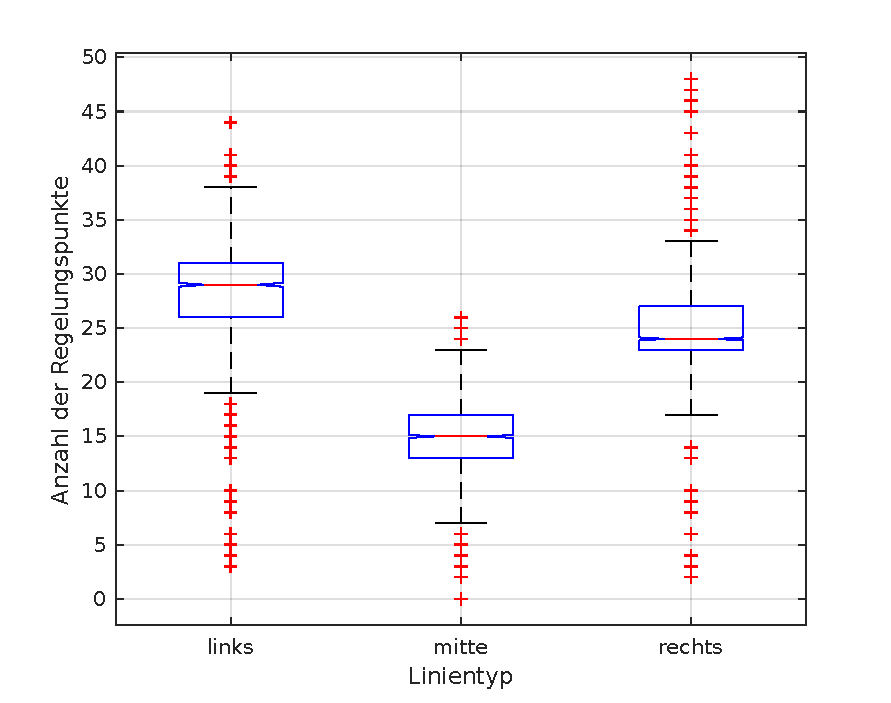
\includegraphics[width=0.9\textwidth]{evaluation_riverflow_regelungspunkte_je_linie_0.2m_s_3Hz.pdf}
	\caption{Alle eingeführten Koordinatensysteme im Überblick}
	\label{fig:evaluation:riverflow:regelungspunkte_je_linie}
\end{figure}